\documentclass[11pt,a4paper]{article}

\usepackage[margin=2.2cm]{geometry}
\usepackage[T1]{fontenc}
\usepackage{lmodern}
\usepackage{amsmath,amssymb}
\usepackage{booktabs}
\usepackage{graphicx}
\usepackage{xcolor}
\usepackage{tikz}
\usetikzlibrary{arrows.meta,positioning,fit,calc,backgrounds}
\usepackage{pgfplots}
\pgfplotsset{compat=1.17}
\usepgfplotslibrary{groupplots}
\usepackage{caption}
\usepackage{subcaption}
\usepackage{enumitem}
\usepackage[section]{placeins}
\usepackage{hyperref}
\hypersetup{colorlinks=true,linkcolor=blue!50!black,urlcolor=blue!50!black,citecolor=blue!50!black}

\definecolor{aa}{HTML}{1F77B4}
\definecolor{glob}{HTML}{D62728}
\definecolor{sift}{HTML}{7F7F7F}
\definecolor{ok}{HTML}{2CA02C}

\title{\textbf{Reproducing VGGT: Visual Geometry Grounded Transformer}\\[4pt]
\large A from-scratch re-implementation, verification against the released model,\\
and a small-scale reproduction of the paper's main claims}
\author{Platinum-Saber/VGGT}
\date{October 2026}

\begin{document}
\maketitle

\begin{abstract}
VGGT (Wang et al., CVPR 2025) is a 1.2\,B-parameter feed-forward transformer that predicts, from one to hundreds of
images, all key 3D attributes of a scene: camera parameters, depth maps, point maps and point tracks.
We re-implemented the camera, depth and point-map branches of VGGT from the paper and verified the implementation
against the official code. With identical weights it reproduces the official outputs \emph{exactly} (maximum absolute
difference $0$), both with randomised weights on CPU and with the released \texttt{VGGT-1B} checkpoint on real images on an
NVIDIA T4. Because retraining the 1\,B model is far beyond the available compute, we additionally trained a 10.7\,M-parameter
VGGT from scratch on procedurally rendered multi-view scenes. At this scale we reproduce three findings of the paper:
(i) Alternating-Attention clearly outperforms global-only attention at equal parameter count,
(ii) point maps obtained from predicted depth and cameras are more accurate than those of the dedicated point head, and
(iii) with sufficient training (15k steps on a GPU) the feed-forward model beats a classical SIFT + 5-point RANSAC baseline in
pose AUC@30, although the classical method remains more precise at tight thresholds.
\end{abstract}

\tableofcontents
\newpage

%==========================================================================================
\section{Introduction}

VGGT~\cite{vggt} replaces the classical, optimisation-heavy structure-from-motion (SfM) pipeline with a single forward
pass of a large transformer. Given $N$ images $(I_i)_{i=1}^N$ it predicts
\begin{equation}
  f\big((I_i)_{i=1}^{N}\big) = \big(\mathbf{g}_i,\, D_i,\, P_i,\, T_i\big)_{i=1}^{N},
\end{equation}
i.e.\ per frame the camera parameters $\mathbf{g}_i$, a depth map $D_i$, a point map $P_i$ expressed in the coordinate frame
of the first camera, and features $T_i$ for point tracking. The paper reports state-of-the-art results on camera pose
estimation, multi-view depth, point-map estimation and tracking, often outperforming optimisation-based methods while
running in under a second.

\paragraph{Goal of this work.} Re-implement VGGT from the paper and the official repository~\cite{vggtcode}, verify the
re-implementation, and reproduce the paper's core results as far as possible with limited compute.

\paragraph{Constraints.} The development sandbox had 4 CPU cores, no GPU, and no access to Hugging Face (where the released
weights are hosted). Experiments with the released weights and the longer training runs were therefore executed on a free
Kaggle GPU instance (NVIDIA Tesla T4). The original model was trained on 17 datasets using 64 A100 GPUs for nine days, so a
full re-training was out of scope; instead we train a scaled-down model on synthetic data and test whether the
paper's qualitative claims hold.

\paragraph{Contributions.}
\begin{enumerate}[leftmargin=*,itemsep=1pt]
  \item A clean re-implementation of VGGT (camera, depth and point heads) whose parameter names match the official
        release, so the released checkpoint loads with \texttt{strict=True}.
  \item A bit-exact verification against the official implementation, with random weights and with the real
        \texttt{VGGT-1B} weights on real images.
  \item A procedural multi-view renderer with exact ground truth, a training/evaluation pipeline implementing the
        paper's losses and metrics, and a classical baseline.
  \item A small-scale reproduction of three claims of the paper, including the Alternating-Attention ablation.
\end{enumerate}

%==========================================================================================
\section{Method}

\subsection{Architecture}

Figure~\ref{fig:arch} summarises the architecture we implemented.

\begin{figure}[t]
\centering
\resizebox{\linewidth}{!}{%
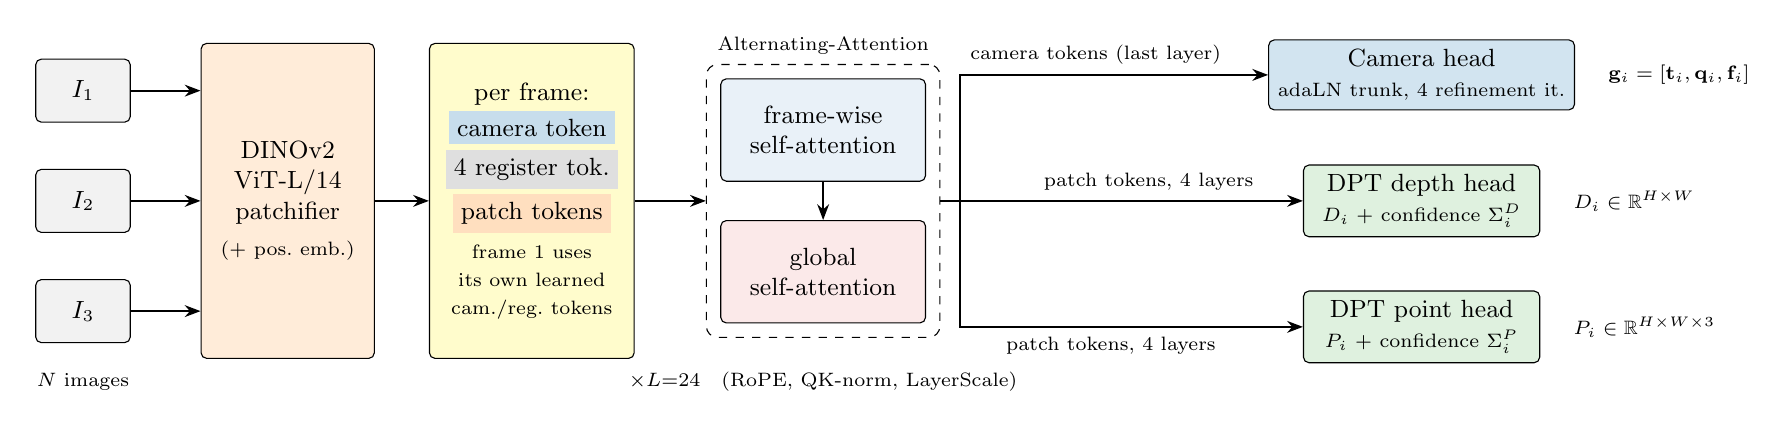
\begin{tikzpicture}[
  font=\small,
  box/.style={draw, rounded corners=2pt, minimum height=8mm, align=center, fill=#1},
  box/.default=white,
  arr/.style={-{Stealth[length=2mm]}, thick},
  lab/.style={font=\scriptsize, align=center}
]
% inputs
\foreach \i/\y in {1/1.4,2/0.0,3/-1.4} {
  \node[box=gray!10, minimum width=12mm] (img\i) at (0,\y) {$I_{\i}$};
}
\node[lab] at (0,-2.3) {$N$ images};
% patchifier
\node[box=orange!15, minimum width=22mm, minimum height=40mm] (dino) at (2.6,0) {DINOv2\\ViT-L/14\\patchifier\\[2pt]\scriptsize(+ pos.\ emb.)};
\foreach \i in {1,2,3} { \draw[arr] (img\i) -- (dino.west |- img\i); }
% tokens
\node[box=yellow!20, minimum width=26mm, minimum height=40mm] (tok) at (5.7,0) {per frame:\\[2pt]
  \colorbox{aa!25}{camera token}\\[1pt]\colorbox{gray!25}{4 register tok.}\\[1pt]\colorbox{orange!25}{patch tokens}\\[3pt]
  \scriptsize frame 1 uses\\[-1pt]\scriptsize its own learned\\[-1pt]\scriptsize cam./reg.\ tokens};
\draw[arr] (dino) -- (tok);
% AA block
\node[box=aa!10, minimum width=26mm, minimum height=13mm] (fa) at (9.4,0.9) {frame-wise\\self-attention};
\node[box=glob!10, minimum width=26mm, minimum height=13mm] (ga) at (9.4,-0.9) {global\\self-attention};
\draw[arr] (fa) -- (ga);
\node[draw, dashed, rounded corners, fit=(fa)(ga), inner sep=5pt, label={[lab]above:Alternating-Attention}] (aa) {};
\node[lab] at (9.4,-2.3) {$\times L{=}24$ \; (RoPE, QK-norm, LayerScale)};
\draw[arr] (tok) -- (aa.west |- tok);
% heads
\node[box=aa!20, minimum width=30mm] (cam) at (17.0,1.6) {Camera head\\\scriptsize adaLN trunk, 4 refinement it.};
\node[box=ok!15, minimum width=30mm] (dep) at (17.0,0) {DPT depth head\\\scriptsize $D_i$ + confidence $\Sigma^D_i$};
\node[box=ok!15, minimum width=30mm] (pts) at (17.0,-1.6) {DPT point head\\\scriptsize $P_i$ + confidence $\Sigma^P_i$};
\coordinate (aaout) at ($(aa.east)+(0.25,0)$);
\draw[thick] (aa.east) -- (aaout);
\draw[arr] (aaout) |- node[lab, pos=0.72, above] {camera tokens (last layer)} (cam.west);
\draw[arr] (aaout) -- node[lab, above, pos=0.55] {patch tokens, 4 layers} (dep.west);
\draw[arr] (aaout) |- node[lab, pos=0.72, below] {patch tokens, 4 layers} (pts.west);
% outputs
\node[lab, right=3mm of cam] (go) {$\mathbf{g}_i=[\mathbf{t}_i,\mathbf{q}_i,\mathbf{f}_i]$};
\node[lab, right=3mm of dep] {$D_i\in\mathbb{R}^{H\times W}$};
\node[lab, right=3mm of pts] {$P_i\in\mathbb{R}^{H\times W\times 3}$};
\end{tikzpicture}}
\caption{VGGT architecture as implemented. Each image is patchified by DINOv2; a camera token and four register tokens are
prepended per frame (the first frame uses distinct learned tokens, defining the world frame). $L{=}24$ Alternating-Attention
layers alternate frame-wise self-attention (tokens attend within their frame) and global self-attention (tokens attend across
all frames). The concatenated frame/global outputs ($2C$ channels) feed a camera head and two DPT dense heads. The tracking head
of the paper was not re-implemented.}
\label{fig:arch}
\end{figure}

\paragraph{Patchifier and tokens.} Images are normalised with ImageNet statistics and patchified by DINOv2 ViT-L/14 with
register tokens (24 blocks, 1024 channels). Positional embeddings are bicubically interpolated to the input aspect ratio.
For every frame, one camera token and four register tokens are concatenated to the patch tokens. Two sets of these
tokens are learned: one for the first frame and one for all others, which identifies the reference frame.

\paragraph{Alternating-Attention (AA).} The aggregator consists of $L=24$ pairs of transformer blocks. A
\emph{frame-wise} block reshapes tokens to $(B\!\cdot\!S, P, C)$ so attention is restricted to one image; a
\emph{global} block reshapes to $(B, S\!\cdot\!P, C)$ so all tokens of all frames attend to each other. Blocks are pre-norm
ViT blocks with 16 heads, 2D rotary position embeddings (RoPE, base frequency 100; special tokens receive position 0),
QK-normalisation and LayerScale ($\gamma_0 = 0.01$). The outputs of the frame and global block of a layer are concatenated to
$2C = 2048$ channels and passed to the heads.

\paragraph{Camera head.} The camera tokens of the last layer are refined iteratively (4 iterations). In each iteration the
current pose estimate (initialised with a learned ``empty'' token) is embedded and used to produce shift, scale and gate
parameters for adaptive layer normalisation of the camera tokens; four self-attention blocks across frames and an MLP
then predict an additive update. The 9-dimensional encoding is
$\mathbf{g} = [\mathbf{t}\in\mathbb{R}^3,\; \mathbf{q}\in\mathbb{R}^4,\; (\text{fov}_h, \text{fov}_w)]$ (translation,
unit quaternion, field of view; principal point at the image centre), with a ReLU on the field of view.

\paragraph{Dense heads.} Two DPT heads~\cite{dpt} read patch tokens from layers $\{4, 11, 17, 23\}$, project and resize them to
four scales ($\times4, \times2, \times1, \times\tfrac12$), fuse them coarse-to-fine and upsample to full resolution. Depth uses
an $\exp$ activation, point maps the inverse-log activation $\operatorname{sign}(y)(e^{|y|}-1)$. A final channel predicts an
aleatoric confidence $\Sigma = 1 + e^{c}$.

\subsection{Training objective}

Following the paper (Sec.~3.4) and the official training code, the loss is
$\mathcal{L} = 5\,\mathcal{L}_\text{camera} + \mathcal{L}_\text{depth} + \mathcal{L}_\text{pmap}$ with
\begin{align}
  \mathcal{L}_\text{camera} &= \frac{1}{K}\sum_{k=1}^{K} \gamma^{K-k}\,\big\|\hat{\mathbf g}^{(k)} - \mathbf g\big\|_1,
     \qquad \gamma = 0.6, \\
  \mathcal{L}_\text{depth} &= \sum_i \Big\| \Sigma^D_i \odot (\hat D_i - D_i)\Big\|
     + \Big\| \Sigma^D_i \odot (\nabla \hat D_i - \nabla D_i)\Big\| - \alpha \log \Sigma^D_i,
     \qquad \alpha = 0.2,
\end{align}
and $\mathcal{L}_\text{pmap}$ defined analogously to $\mathcal{L}_\text{depth}$. The paper states a Huber loss for the camera; the official
code uses L1, which we follow. As in the official code, the plain (unweighted) regression term is added and the 2\% largest
per-pixel errors are discarded. Ground truth is normalised so that the first camera is the world frame and the mean
distance of all valid 3D points to the origin is 1.

\subsection{Evaluation metrics}
\begin{itemize}[leftmargin=*,itemsep=1pt]
  \item \textbf{Camera pose:} for every ordered pair of frames, the relative rotation error (RRA) and the angle between
        relative translation directions (RTA), in degrees. AUC@$\tau$ is the area under the accuracy curve of
        $\max(\text{RRA},\text{RTA})$ for thresholds $1,\dots,\tau$ degrees. We also report RRA@15/RTA@15 (fraction
        below $15^\circ$) and median errors.
  \item \textbf{Depth:} AbsRel and $\delta < 1.25$ after one median scale per sequence.
  \item \textbf{Point maps:} mean Euclidean error after a least-squares similarity (Umeyama) alignment, in normalised
        scene units.
\end{itemize}

%==========================================================================================
\section{Verification of the implementation}
\label{sec:verify}

\subsection{Numerical equivalence with the official code}

Parameter names were chosen to match the official release, so a state dict can be moved between the two implementations
with \texttt{load\_state\_dict(strict=True)}. We performed two equivalence tests (Table~\ref{tab:equiv}).

\begin{enumerate}[leftmargin=*,itemsep=1pt]
  \item \textbf{Random weights, CPU} (\texttt{tests/test\_equivalence.py}): a reduced configuration (DINOv2-S patchifier,
        4 AA layers, 2-block camera trunk) with \emph{all} parameters randomised, on non-square input ($182\times252$, 3 frames),
        which exercises positional-embedding interpolation, RoPE, AA, the camera trunk and both DPT heads.
  \item \textbf{Released weights, GPU}: the full \texttt{facebook/VGGT-1B} checkpoint loaded into both implementations,
        evaluated in fp32 on the first 8 images of the official \texttt{examples/kitchen} scene on a Tesla T4.
\end{enumerate}

\begin{table}[htbp]
\centering
\caption{Maximum absolute difference between the official implementation and ours with identical weights.}
\label{tab:equiv}
\begin{tabular}{lccc}
\toprule
Output & Random weights (CPU) & \texttt{VGGT-1B}, real images (T4) & $\max|\text{ref}|$ (T4)\\
\midrule
Pose encoding $\mathbf g$          & 0.0 & 0.0 & 1.36 \\
Depth $D$                          & 0.0 & 0.0 & 3.57 \\
Depth confidence $\Sigma^D$        & 0.0 & 0.0 & 30.3 \\
Point map $P$                      & 0.0 & 0.0 & 2.86 \\
Point confidence $\Sigma^P$        & 0.0 & 0.0 & 31.6 \\
\bottomrule
\end{tabular}
\end{table}

\noindent The implementation is therefore functionally identical to the released model: every number the paper reports
for the camera, depth and point branches of VGGT-1B is produced unchanged by this code.

\paragraph{A subtle detail.} A first version differed by up to $5\times10^{-3}$ in the DPT outputs. The cause is the
residual unit of the official DPT head, which applies an \emph{in-place} ReLU to its input before the skip connection; the
skip path therefore carries $\operatorname{relu}(x)$ rather than $x$. The released weights were trained with this behaviour,
so it must be replicated.

\paragraph{Model size.} The default configuration has $1.19$\,B parameters; the official model has $1.26$\,B, the difference
being the tracking head that we did not re-implement.

\subsection{Inference cost with the released weights}

Table~\ref{tab:timing} and Figure~\ref{fig:timing} report wall-clock time and peak GPU memory of our implementation with the
released weights on a Tesla T4 (fp16 autocast, images 518\,px wide). Peak memory includes $\approx$4.7\,GiB of fp32 weights;
the 1-frame measurement includes GPU warm-up. Time grows super-linearly beyond 8 frames because global attention is
quadratic in the total number of tokens.

\begin{table}[htbp]
\centering
\caption{Inference time and peak memory, our implementation with \texttt{VGGT-1B} weights, Tesla T4.}
\label{tab:timing}
\begin{tabular}{lcccccc}
\toprule
Frames & 1 & 2 & 4 & 8 & 16 & 32 \\
\midrule
Time (s)               & 0.76 & 0.59 & 1.05 & 2.21 & 5.56 & 15.68 \\
Peak GPU memory (GiB)  & 7.2  & 7.3  & 7.9  & 8.9  & 9.2  & 9.8 \\
\bottomrule
\end{tabular}
\end{table}

\begin{figure}[htbp]
\centering
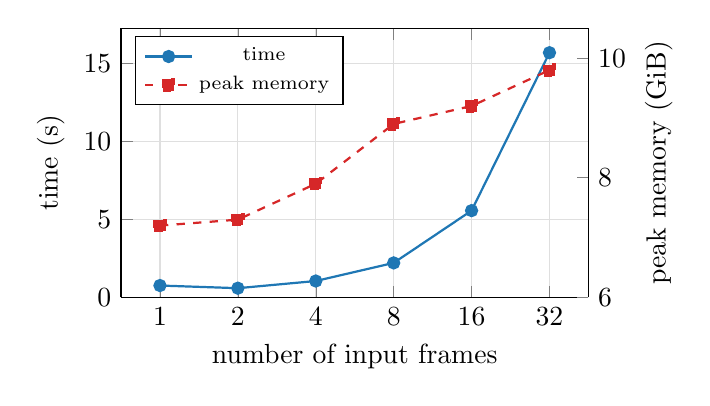
\begin{tikzpicture}
\begin{axis}[
  width=0.62\linewidth, height=5cm,
  xmode=log, log basis x=2, xtick={1,2,4,8,16,32}, xticklabels={1,2,4,8,16,32},
  xlabel={number of input frames}, ylabel={time (s)}, ymin=0,
  axis y line*=left, grid=major, grid style={gray!25}, legend style={at={(0.03,0.97)},anchor=north west,font=\scriptsize}
]
\addplot[aa, thick, mark=*] coordinates {(1,0.76) (2,0.59) (4,1.05) (8,2.21) (16,5.56) (32,15.68)};
\addlegendentry{time}
\addlegendimage{glob, thick, mark=square*, dashed}\addlegendentry{peak memory}
\end{axis}
\begin{axis}[
  width=0.62\linewidth, height=5cm,
  xmode=log, log basis x=2, xtick=\empty,
  ylabel={peak memory (GiB)}, ymin=6, ymax=10.5,
  axis y line*=right, axis x line=none
]
\addplot[glob, thick, mark=square*, dashed] coordinates {(1,7.2) (2,7.3) (4,7.9) (8,8.9) (16,9.2) (32,9.8)};
\end{axis}
\end{tikzpicture}
\caption{Inference scaling of VGGT-1B (our implementation) on a Tesla T4.}
\label{fig:timing}
\end{figure}

\noindent Exporting the 25-image kitchen scene with \texttt{scripts/demo\_pretrained.py} produced 25 depth maps and a
coloured point cloud of 2.27\,M points (unprojected predicted depth with predicted cameras, top-50\% confidence).

%==========================================================================================
\section{Small-scale reproduction by training from scratch}

\subsection{Synthetic multi-view data}

Since none of the 17 training datasets of the paper were available, we wrote a procedural ray-caster
(\texttt{training/synthetic.py}). Each scene is a closed room (inward-facing walls) with 3--6 random spheres and boxes.
Surfaces have solid, i.e.\ 3D-consistent, textures (per-object colour, sinusoidal bands, checkerboards) with fixed Lambertian
shading, so appearance is consistent across views and supports matching. Cameras are placed on an arc around the scene centre
($30$--$100^\circ$ spread) looking at a jittered target, with field of view $50$--$75^\circ$. Each view is $112\times112$
pixels and comes with exact depth, points, intrinsics and extrinsics. We rendered 3{,}000 training scenes with 6 views each, and
200 held-out test scenes from a different random seed; evaluation uses the first 2, 4 or 6 views of each test scene.
Figure~\ref{fig:qual} shows examples.

\subsection{Models and training setup}

\begin{table}[htbp]
\centering
\caption{Training configurations. Both models share the data, losses and optimiser and have the same parameter count.}
\label{tab:setup}
\begin{tabular}{lcc}
\toprule
 & Alternating-Attention (AA) & Global-only (ablation) \\
\midrule
Patchifier & \multicolumn{2}{c}{conv $14\times14$ (no DINOv2 pre-training)} \\
Width / heads & \multicolumn{2}{c}{$C=192$ / 6} \\
Aggregator & 6 frame + 6 global blocks & 12 global blocks \\
Heads & \multicolumn{2}{c}{camera (2-block trunk), 2 light DPT heads (32 features)} \\
Parameters & 10.66\,M & 10.66\,M \\
\midrule
Optimiser & \multicolumn{2}{c}{AdamW, lr $4\!\times\!10^{-4}$, wd 0.05, warm-up + cosine, grad.\ clip 1} \\
Frames per sample & \multicolumn{2}{c}{2--6 (random per batch)} \\
Run A (CPU, 2 threads) & \multicolumn{2}{c}{batch 8, 3{,}000 steps ($\approx$2.5\,h per model)} \\
Run B (Kaggle T4) & \multicolumn{2}{c}{batch 16, 15{,}000 steps (10$\times$ more samples)} \\
\bottomrule
\end{tabular}
\end{table}

The global-only model is the paper's ``global self-attention only'' ablation (Table~5 of~\cite{vggt}); we doubled the number of global
blocks so both models have exactly the same parameter budget. As a classical reference we use SIFT features, a ratio test and the
5-point algorithm with RANSAC (OpenCV) on every frame pair, \emph{given the ground-truth intrinsics}; pairs where it fails count as
$180^\circ$ error.

%==========================================================================================
\section{Results}

\subsection{Camera pose}

Table~\ref{tab:pose} lists the pose metrics with 4 input frames for both training lengths, and Figure~\ref{fig:pose} visualises the
main comparisons.

\begin{table}[htbp]
\centering
\caption{Camera pose on 200 held-out scenes (4 frames, 12 ordered pairs per scene). Best per column in bold.}
\label{tab:pose}
\setlength{\tabcolsep}{4pt}
\resizebox{\linewidth}{!}{%
\begin{tabular}{llccccccc}
\toprule
Method & Training & AUC@30$\uparrow$ & AUC@15$\uparrow$ & AUC@5$\uparrow$ & RRA@15$\uparrow$ & RTA@15$\uparrow$ & med.\ rot.$\downarrow$ & med.\ transl.$\downarrow$\\
\midrule
SIFT + 5-pt RANSAC$^\dagger$ & -- & 0.206 & \textbf{0.135} & \textbf{0.050} & 0.583 & 0.226 & 10.4$^\circ$ & 69.6$^\circ$ \\
\midrule
Global-only & 3k, CPU  & 0.003 & 0.000 & 0.000 & 0.228 & 0.002 & 25.3$^\circ$ & 91.7$^\circ$ \\
AA          & 3k, CPU  & 0.042 & 0.011 & 0.000 & 0.377 & 0.038 & 19.4$^\circ$ & 67.8$^\circ$ \\
\midrule
Global-only & 15k, GPU & 0.003 & 0.000 & 0.000 & 0.231 & 0.002 & 25.3$^\circ$ & 92.4$^\circ$ \\
AA          & 15k, GPU & \textbf{0.270} & 0.082 & 0.004 & \textbf{0.865} & \textbf{0.269} & \textbf{7.0}$^\circ$ & \textbf{23.6}$^\circ$ \\
\bottomrule
\multicolumn{9}{l}{\footnotesize $^\dagger$ uses ground-truth intrinsics; fails (no pose) on 21.6\% of pairs. VGGT models never fail.}
\end{tabular}}
\end{table}

\begin{figure}[htbp]
\centering
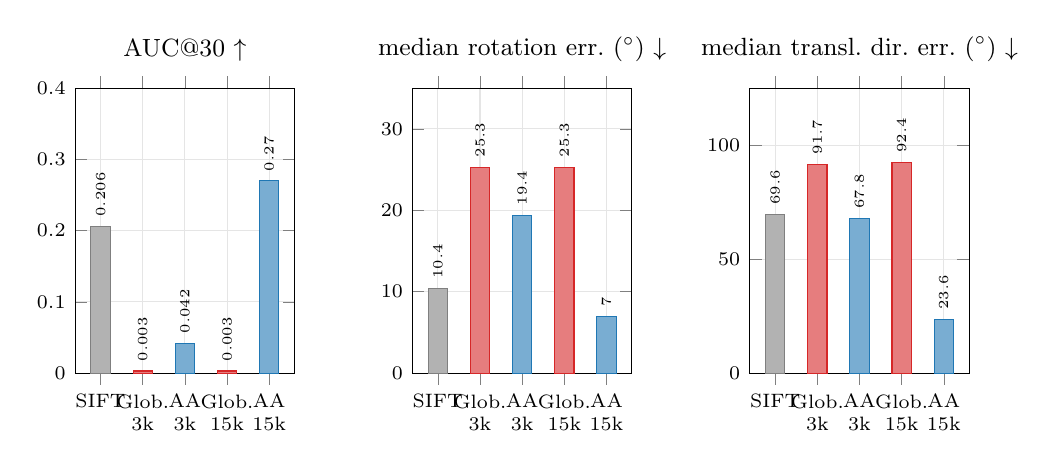
\begin{tikzpicture}
\begin{groupplot}[
  group style={group size=3 by 1, horizontal sep=1.5cm},
  width=0.36\linewidth, height=5.2cm, ybar, /pgf/bar width=7pt,
  symbolic x coords={SIFT,Glob3k,AA3k,Glob15k,AA15k},
  xtick={SIFT,Glob3k,AA3k,Glob15k,AA15k}, xticklabels={SIFT,Glob.\\3k,AA\\3k,Glob.\\15k,AA\\15k}, /pgf/bar shift=0pt,
  xticklabel style={font=\scriptsize, align=center}, tick label style={font=\scriptsize},
  ymin=0, enlarge x limits=0.15, nodes near coords, every node near coord/.append style={font=\tiny, rotate=90, anchor=west, /pgf/number format/fixed, /pgf/number format/precision=3},
  grid=major, grid style={gray!20}, title style={font=\small}
]
\nextgroupplot[title={AUC@30 $\uparrow$}, ymax=0.4]
\addplot[fill=sift!60, draw=sift] coordinates {(SIFT,0.206)};
\addplot[fill=glob!60, draw=glob] coordinates {(Glob3k,0.003) (Glob15k,0.003)};
\addplot[fill=aa!60, draw=aa] coordinates {(AA3k,0.042) (AA15k,0.270)};
\nextgroupplot[title={median rotation err.\ ($^\circ$) $\downarrow$}, ymax=35]
\addplot[fill=sift!60, draw=sift] coordinates {(SIFT,10.4)};
\addplot[fill=glob!60, draw=glob] coordinates {(Glob3k,25.3) (Glob15k,25.3)};
\addplot[fill=aa!60, draw=aa] coordinates {(AA3k,19.4) (AA15k,7.0)};
\nextgroupplot[title={median transl.\ dir.\ err.\ ($^\circ$) $\downarrow$}, ymax=125]
\addplot[fill=sift!60, draw=sift] coordinates {(SIFT,69.6)};
\addplot[fill=glob!60, draw=glob] coordinates {(Glob3k,91.7) (Glob15k,92.4)};
\addplot[fill=aa!60, draw=aa] coordinates {(AA3k,67.8) (AA15k,23.6)};
\end{groupplot}
\end{tikzpicture}
\caption{Pose accuracy with 4 frames. Grey: classical baseline; red: global-only attention; blue: Alternating-Attention.
A median translation-direction error of $\approx 90^\circ$ corresponds to chance.}
\label{fig:pose}
\end{figure}

Table~\ref{tab:frames} and Figure~\ref{fig:auc} show how pose accuracy depends on the number of input frames.

\begin{table}[htbp]
\centering
\caption{Effect of the number of input frames (15k-step GPU models).}
\label{tab:frames}
\begin{tabular}{lcccccc}
\toprule
 & \multicolumn{3}{c}{AA} & \multicolumn{3}{c}{Global-only} \\
\cmidrule(lr){2-4}\cmidrule(lr){5-7}
Frames & 2 & 4 & 6 & 2 & 4 & 6 \\
\midrule
AUC@30 $\uparrow$           & 0.249 & 0.270 & 0.272 & 0.005 & 0.003 & 0.004 \\
RRA@15 $\uparrow$           & 0.860 & 0.865 & 0.872 & 0.270 & 0.231 & 0.235 \\
RTA@15 $\uparrow$           & 0.255 & 0.269 & 0.276 & 0.000 & 0.002 & 0.003 \\
Median rot.\ err.\ $\downarrow$  & 7.7$^\circ$ & 7.0$^\circ$ & 7.2$^\circ$ & 23.0$^\circ$ & 25.3$^\circ$ & 24.9$^\circ$ \\
Median transl.\ err.\ $\downarrow$ & 26.1$^\circ$ & 23.6$^\circ$ & 23.8$^\circ$ & 91.6$^\circ$ & 92.4$^\circ$ & 91.1$^\circ$ \\
Focal rel.\ err.\ $\downarrow$  & 0.100 & 0.094 & 0.089 & 0.115 & 0.119 & 0.121 \\
\bottomrule
\end{tabular}
\end{table}

\begin{figure}[htbp]
\centering
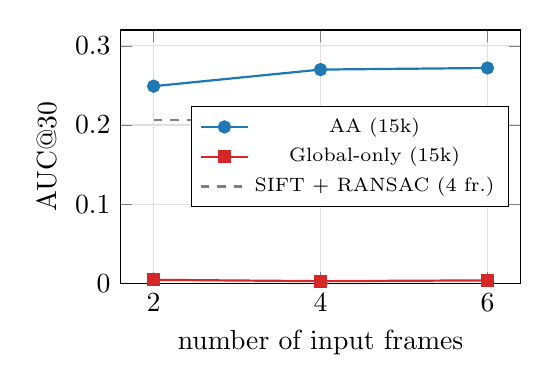
\begin{tikzpicture}
\begin{axis}[
  width=0.55\linewidth, height=4.8cm, xlabel={number of input frames}, ylabel={AUC@30},
  xtick={2,4,6}, ymin=0, ymax=0.32, grid=major, grid style={gray!25},
  legend style={at={(0.97,0.5)},anchor=east,font=\scriptsize}
]
\addplot[aa, thick, mark=*] coordinates {(2,0.249) (4,0.270) (6,0.272)}; \addlegendentry{AA (15k)}
\addplot[glob, thick, mark=square*] coordinates {(2,0.0045) (4,0.0028) (6,0.0038)}; \addlegendentry{Global-only (15k)}
\addplot[sift, thick, dashed, domain=2:6] {0.206}; \addlegendentry{SIFT + RANSAC (4 fr.)}
\end{axis}
\end{tikzpicture}
\caption{Pose AUC@30 versus number of input frames. The AA model improves slightly with more frames.}
\label{fig:auc}
\end{figure}

\FloatBarrier
\subsection{Depth and point maps}

\begin{table}[htbp]
\centering
\caption{Depth and point-map accuracy (4 frames). Point errors in normalised scene units after Sim(3) alignment.}
\label{tab:dense}
\begin{tabular}{llcccc}
\toprule
Model & Training & AbsRel $\downarrow$ & $\delta<1.25$ $\uparrow$ & Point head $\downarrow$ & Depth + camera $\downarrow$ \\
\midrule
Global-only & 3k, CPU  & 0.218 & 0.857 & 0.250 & 0.251 \\
AA          & 3k, CPU  & 0.233 & 0.848 & 0.254 & \textbf{0.235} \\
\midrule
Global-only & 15k, GPU & 0.087 & 0.937 & 0.110 & 0.212 \\
AA          & 15k, GPU & 0.087 & 0.937 & 0.099 & \textbf{0.096} \\
\bottomrule
\end{tabular}
\end{table}

\begin{figure}[htbp]
\centering
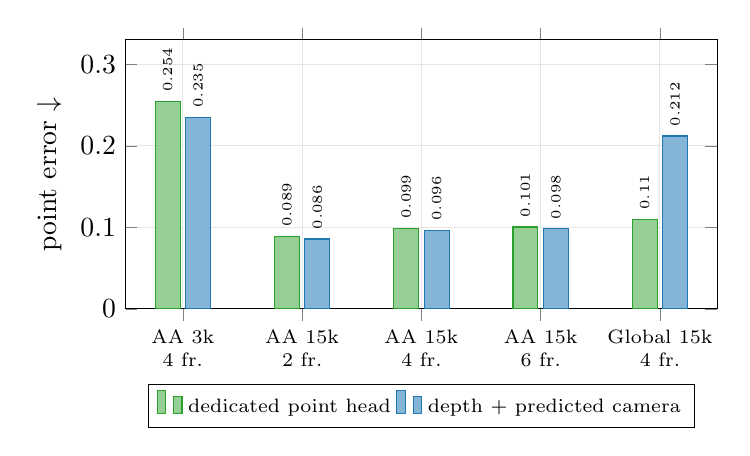
\begin{tikzpicture}
\begin{axis}[
  width=0.75\linewidth, height=5cm, ybar, /pgf/bar width=9pt,
  symbolic x coords={AA3k-4,AA15k-2,AA15k-4,AA15k-6,G15k-4},
  xtick=data, xticklabels={AA 3k\\4 fr., AA 15k\\2 fr., AA 15k\\4 fr., AA 15k\\6 fr., Global 15k\\4 fr.},
  xticklabel style={font=\scriptsize, align=center},
  ylabel={point error $\downarrow$}, ymin=0, ymax=0.33, enlarge x limits=0.12,
  legend style={at={(0.5,-0.28)},anchor=north,legend columns=2,font=\scriptsize},
  nodes near coords, every node near coord/.append style={font=\tiny, rotate=90, anchor=west, /pgf/number format/fixed, /pgf/number format/precision=3},
  grid=major, grid style={gray!20}
]
\addplot[fill=ok!50, draw=ok] coordinates {(AA3k-4,0.254) (AA15k-2,0.0885) (AA15k-4,0.0986) (AA15k-6,0.1005) (G15k-4,0.110)};
\addplot[fill=aa!55, draw=aa] coordinates {(AA3k-4,0.235) (AA15k-2,0.0857) (AA15k-4,0.0964) (AA15k-6,0.0981) (G15k-4,0.212)};
\legend{dedicated point head, depth + predicted camera}
\end{axis}
\end{tikzpicture}
\caption{Point maps from the point head versus unprojecting predicted depth with predicted cameras. For the AA model the
depth + camera combination is consistently (slightly) better; for the global-only model, whose cameras are poor, it is much worse.}
\label{fig:points}
\end{figure}

\FloatBarrier
\subsection{Training dynamics and qualitative results}

\begin{figure}[htbp]
\centering
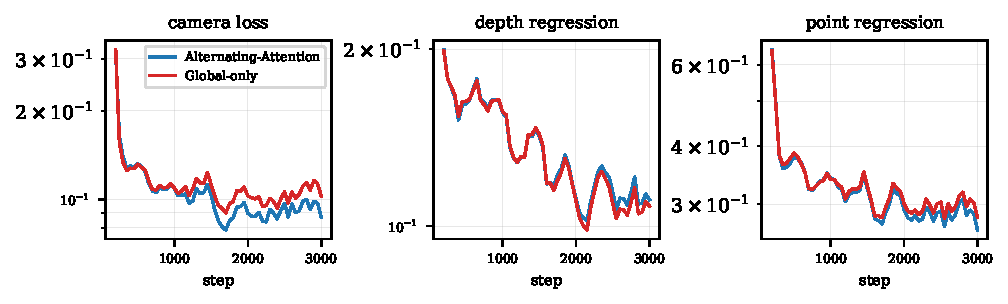
\includegraphics[width=\linewidth]{figures/training_curves.pdf}
\caption{Training losses of the 3k-step CPU runs (moving average, log scale). Depth and point losses are almost identical for
both models, while the AA model reaches a lower camera loss. The camera loss was still decreasing at the end of training,
which motivated the longer GPU run.}
\label{fig:curves}
\end{figure}

\begin{figure}[htbp]
\centering
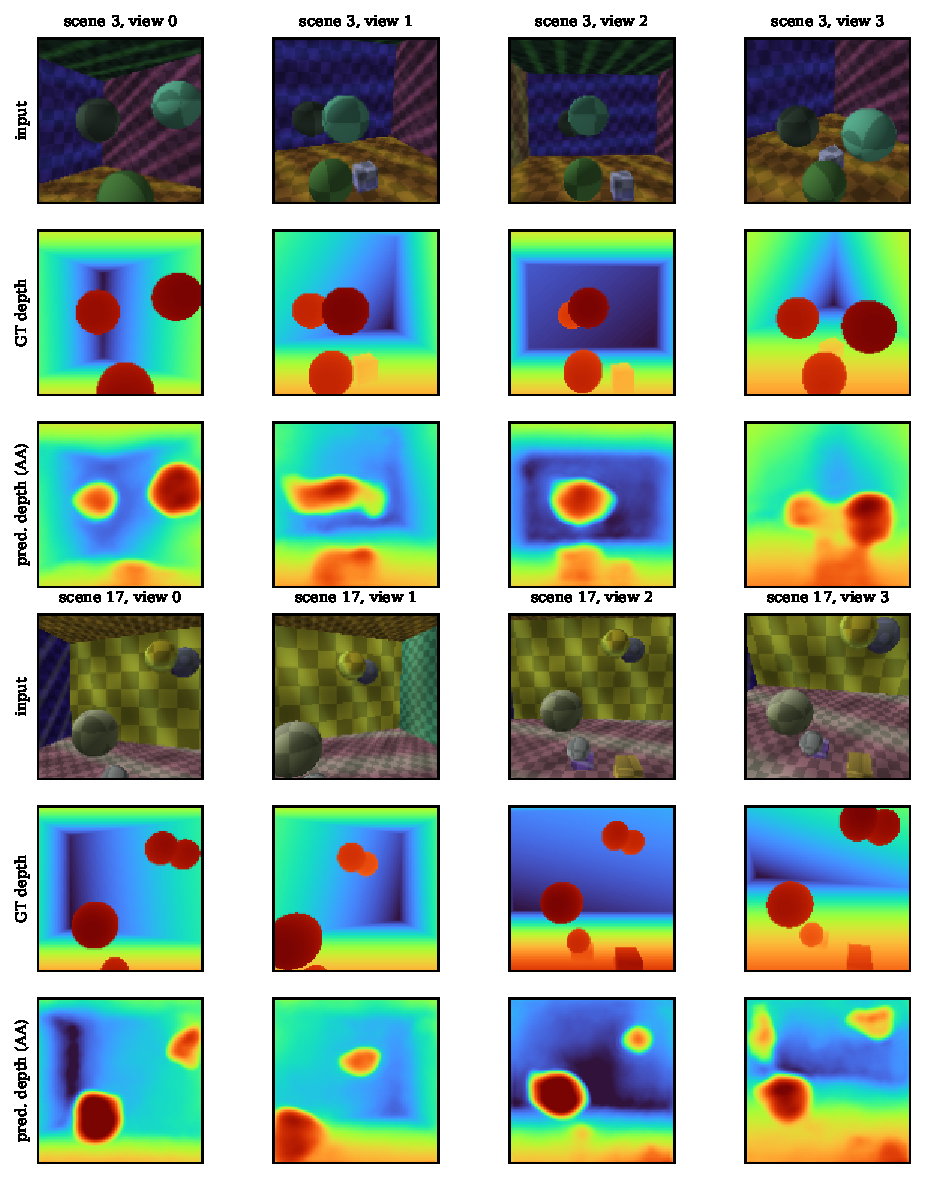
\includegraphics[width=0.92\linewidth]{figures/qualitative_depth.pdf}
\caption{Two held-out synthetic scenes (4 views each): input images, ground-truth depth, and depth predicted by the 3k-step
CPU AA model (median-scaled; same colour range as the ground truth).}
\label{fig:qual}
\end{figure}

%==========================================================================================
\section{Discussion}

Table~\ref{tab:claims} relates our findings to the claims of the paper.

\begin{table}[htbp]
\centering
\caption{Claims of the paper and their status in this reproduction.}
\label{tab:claims}
\renewcommand{\arraystretch}{1.25}
\begin{tabular}{p{4.6cm}p{8.0cm}p{2.0cm}}
\toprule
Claim (paper) & Evidence here & Status \\
\midrule
Released model / architecture as described (Sec.~3) &
Bit-exact outputs vs.\ official code with random and with released weights (Table~\ref{tab:equiv}) & Reproduced \\
Alternating-Attention outperforms global-only attention (Table~5) &
Equal-size models: AUC@30 0.270 vs 0.003; global-only stays at chance for translation even with 5$\times$ more training & Reproduced \\
Depth + camera gives better point maps than the point head (Table~3) &
AA: better at all frame counts and both training lengths (small margin, e.g.\ 0.096 vs 0.099) & Reproduced \\
Feed-forward poses competitive with / better than classical methods (Tables~1--2) &
AUC@30 0.270 vs 0.206 for SIFT+RANSAC with GT intrinsics; SIFT more precise at AUC@5 / AUC@15 & Partially \\
Fast inference (Table~9) &
Sub-second to seconds for 1--16 frames on a T4 (Table~\ref{tab:timing}); not comparable to the paper's H100 numbers & Consistent \\
\bottomrule
\end{tabular}
\end{table}

\paragraph{Why Alternating-Attention matters.} Depth quality is identical for both models (AbsRel 0.087), indicating that depth
on these scenes is largely a single-view problem. The difference lies entirely in cross-view reasoning: the global-only
model never learns relative translation (median error $\approx 92^\circ$, chance level) and only coarse rotation, whereas the AA
model improves steadily with training. Frame-wise attention gives each image a place to build per-frame features before they are
mixed globally, which appears to make correspondence-based reasoning much easier to learn. This matches the paper's ablation.

\paragraph{Training length.} After 3k CPU steps the AA model's camera estimates were weak (AUC@30 0.042) and equally weak on training
scenes, i.e.\ the model was under-trained rather than over-fitting. With 10$\times$ more training samples AUC@30 rose to 0.270.
The camera branch is clearly the slowest to train; the paper's model additionally benefits from DINOv2 initialisation.

\paragraph{Feed-forward versus classical.} The trained model is robust---it always outputs a pose and has much lower median errors---but
its estimates are less precise at tight thresholds than SIFT + RANSAC whenever the latter succeeds (AUC@5 0.004 vs 0.050).
The paper makes a similar observation at full scale: VGGT's feed-forward predictions are already strong, and refining them
with bundle adjustment improves accuracy further.

\paragraph{Limitations.}
\begin{itemize}[leftmargin=*,itemsep=1pt]
  \item One training run (seed) per configuration; differences of a few thousandths (e.g.\ point head vs depth + camera) should be
        read as consistent trends across frame counts rather than statistically established gaps.
  \item A synthetic indoor domain at $112\times112$ pixels, not the paper's real-world benchmarks (CO3D, RealEstate10K, DTU, ETH3D).
  \item A 10.7\,M-parameter model without DINOv2 pre-training, versus 1.2\,B parameters in the paper.
  \item A two-view classical baseline instead of full SfM pipelines (COLMAP, VGGSfM); the baseline is given ground-truth intrinsics.
  \item The tracking head and bundle-adjustment post-processing were not re-implemented.
\end{itemize}

%==========================================================================================
\section{Conclusion}

We re-implemented VGGT's camera, depth and point-map prediction from the paper and showed that the implementation is numerically
identical to the official one---bit-exact with randomised weights and with the released 1.2\,B-parameter checkpoint on real
images on a GPU. It can therefore be used as a drop-in replacement for these branches of the released model.

Training a 10.7\,M-parameter version from scratch on procedurally rendered scenes reproduced the paper's central design finding:
at equal parameter count, Alternating-Attention learns multi-view camera geometry, whereas global-only attention does not
(AUC@30 0.270 vs 0.003). It also reproduced the finding that point maps derived from predicted depth and cameras are more accurate
than directly regressed point maps. With enough training, the small feed-forward model surpassed a classical SIFT + RANSAC
baseline in AUC@30 and in median rotation and translation error, while remaining less precise at tight thresholds---consistent with
the paper's observation that feed-forward predictions benefit from optimisation-based refinement.

Natural next steps are evaluating the released VGGT-1B on a public benchmark (e.g.\ CO3D or RealEstate10K camera AUC) with this
implementation, adding DINOv2 initialisation and longer training to the small model, running several seeds, and re-implementing the
tracking head.

\paragraph{Reproducibility.} All code, configurations, logs and result files are in the repository:
\texttt{vggt/} (model), \texttt{training/} (data, losses, metrics, training, evaluation, baseline), \texttt{tests/} (equivalence test),
\texttt{notebooks/kaggle\_pretrained\_vggt.ipynb} (released-weights experiments and GPU training), \texttt{results/} (JSON results and
training logs), and \texttt{scripts/make\_report\_figures.py} (figures of this report).

\begin{thebibliography}{9}
\bibitem{vggt} J.~Wang, M.~Chen, N.~Karaev, A.~Vedaldi, C.~Rupprecht, D.~Novotny.
  \newblock VGGT: Visual Geometry Grounded Transformer.
  \newblock In \emph{CVPR}, 2025. \url{https://arxiv.org/abs/2503.11651}
\bibitem{vggtcode} Official VGGT implementation. \url{https://github.com/facebookresearch/vggt}
\bibitem{dpt} R.~Ranftl, A.~Bochkovskiy, V.~Koltun. Vision Transformers for Dense Prediction. In \emph{ICCV}, 2021.
\bibitem{dinov2} M.~Oquab et al. DINOv2: Learning Robust Visual Features without Supervision. \emph{TMLR}, 2024.
\end{thebibliography}

\end{document}
